\documentclass[a4paper,12pt,oneside]{book}
\usepackage{polski}
\usepackage[utf8]{inputenc}
\usepackage{graphicx}
\graphicspath{{./images}}
\usepackage[shortlabels]{enumitem}
\usepackage{amssymb}
\usepackage{amsmath}
\usepackage{indentfirst}
\usepackage{pdfpages}

\usepackage{tikz}
%\usepackage{etoolbox} % for \ifthen
\usepackage{listofitems} % for \readlist to create arrays
\usetikzlibrary{arrows.meta} % for arrow size
\usepackage[outline]{contour} % glow around text
\contourlength{1.4pt}
\usepackage[margin=1in]{geometry}
\usepackage{listings}
\usepackage{booktabs}
\usepackage{tabularx}


\tikzset{>=latex} % for LaTeX arrow head
\usepackage{xcolor}
\colorlet{myred}{red!80!black}
\colorlet{myblue}{blue!80!black}
\colorlet{mygreen}{green!60!black}
\colorlet{myorange}{orange!70!red!60!black}
\colorlet{mydarkred}{red!30!black}
\colorlet{mydarkblue}{blue!40!black}
\colorlet{mydarkgreen}{green!30!black}
\tikzstyle{node}=[thick,circle,draw=myblue,minimum size=22,inner sep=0.5,outer sep=0.6]
\tikzstyle{node in}=[node,green!20!black,draw=mygreen!30!black,fill=mygreen!25]
\tikzstyle{node hidden}=[node,blue!20!black,draw=myblue!30!black,fill=myblue!20]
\tikzstyle{node convol}=[node,orange!20!black,draw=myorange!30!black,fill=myorange!20]
\tikzstyle{node out}=[node,red!20!black,draw=myred!30!black,fill=myred!20]
\tikzstyle{connect}=[thick,mydarkblue] %,line cap=round
\tikzstyle{connect arrow}=[-{Latex[length=4,width=3.5]},thick,mydarkblue,shorten <=0.5,shorten >=1]
\tikzset{ % node styles, numbered for easy mapping with \nstyle
	node 1/.style={node in},
	node 2/.style={node hidden},
	node 3/.style={node out},
}
\def\nstyle{int(\lay<\Nnodlen?min(2,\lay):3)} % map layer number onto 1, 2, or 3

\def\shrug{\texttt{\raisebox{0.75em}{\char`\_}\char`\\\char`\_\kern-0.5ex(\kern-0.25ex\raisebox{0.25ex}{\rotatebox{45}{\raisebox{-.75ex}"\kern-1.5ex\rotatebox{-90})}}\kern-0.5ex)\kern-0.5ex\char`\_/\raisebox{0.75em}{\char`\_}}}

\renewcommand\thechapter{\Roman{chapter}}
\renewcommand\thesection{\arabic{section}}
\renewcommand\thesubsection{\thesection.\arabic{subsection}}

\begin{document}

	
\includepdf{Odpowiedz-cover-page.pdf}

	\tableofcontents
	\newpage
	
	\chapter{Pytania - dr. hab. Bogdan Księżopolski}
			\section{Protokoły TCP i UDP - porównanie i zastosowanie.}
			
				\subsubsection*{TCP}
				
				Protokół TCP lub Transmission Control Protocol jest protokołem zorientowanym na połączenie, znajdującym się w warstwie transportowej modelu TCP / IP. Nawiązuje połączenie między komputerem źródłowym a docelowym przed rozpoczęciem komunikacji.
				
				\begin{figure}[h!]
					\centering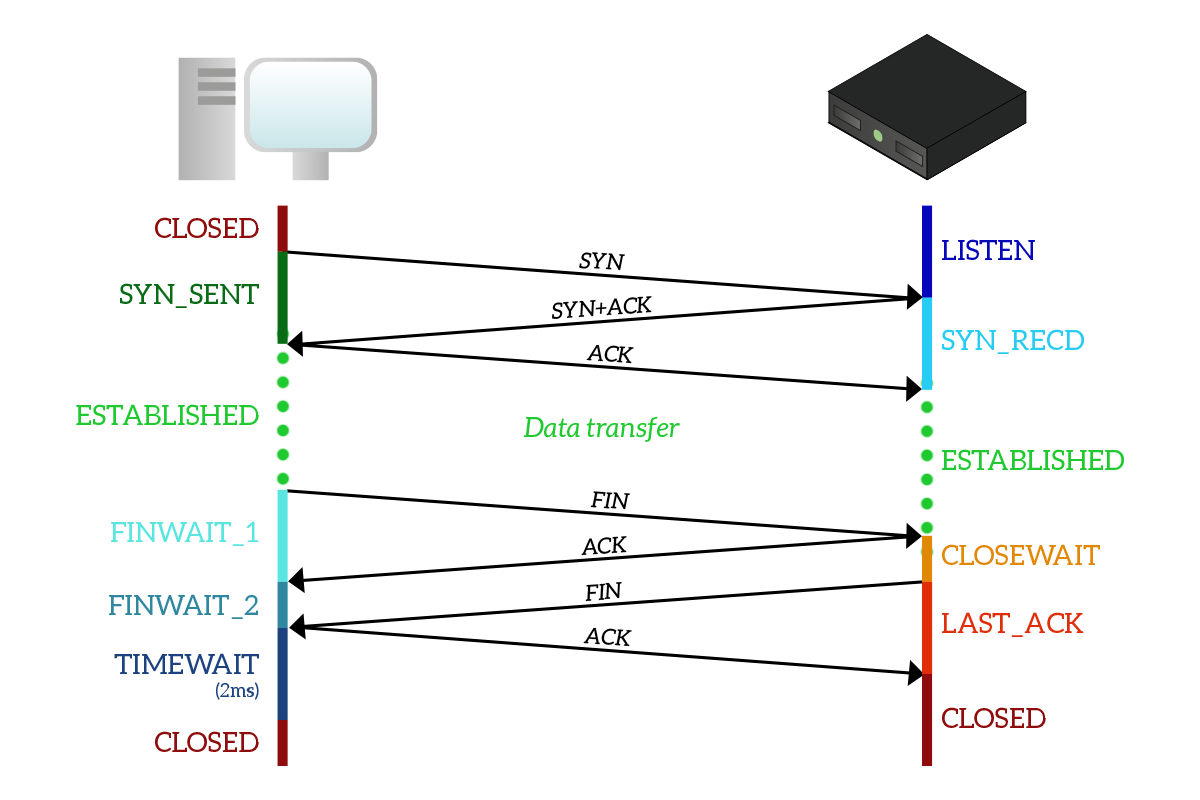
\includegraphics[scale=0.30]{tcp.png}
					\caption{TCP}
				\end{figure}
				
				Jest wysoce niezawodny, ponieważ wykorzystuje 3-drożną kontrolę uzgadniania, przepływu, błędu i przeciążenia. Zapewnia to, że dane wysyłane z komputera źródłowego są dokładnie odbierane przez komputer docelowy. Jeśli w przypadku, otrzymane dane nie są w odpowiednim formacie, to TCP ponownie przesyła dane.
				Poniższe protokoły używają TCP do transmisji danych:
				\begin{itemize}
					\item HTTP
					\item HTTPs
					\item FTP
					\item SMTP
				\end{itemize}
				
				\subsubsection*{UDP}
				
				\begin{figure}[h!]
					\centering
\includegraphics[scale=0.25]{udp.jpg}
					\caption{UDP :D}
				\end{figure}
				
				Protokół UDP lub User Datagram Protocol to bezpołączeniowy protokół znajdujący się w warstwie transportowej modelu TCP / IP. Nie ustanawia połączenia ani nie sprawdza, czy komputer docelowy jest gotowy do odbioru, czy też nie, po prostu przesyła dane bezpośrednio. Protokół UDP służy do przesyłania danych z większą szybkością. Jest mniej niezawodny i dlatego jest używany do przesyłania danych, takich jak pliki audio i wideo.
				UDP nie gwarantuje ani dostarczenia danych, ani nie przesyła utraconych pakietów.	
				
							
			
			\newpage\section{Protokół IP.}
				\subsubsection{IP (Internet Protocol)}
				Protokół internetowy jest protokołem komunikacyjnym warstwy Internet w modelu TCP/IP (odpowiada warstwie sieciowej modelu OSI). Protokół ten definiuje zasady i sposoby postępowania urządzeń sieciowych w celu nawiązania połączenia, utrzymania go i samej transmisji danych. Protokół IP stosowany jest w większości rodzajów sieci, w tym w sieci lokalnej i sieci Internet (każdy host, np. komputer, posiada swój własny, unikalny dla sieci adres IP).
				
				Dane z użyciem protokołu IP transmitowane są w pakietach (paczkach danych). Nie gwarantuje on jednak dotarcia danych do celu czy utrzymania kolejności pakietów. Może się zdążyć, ze odbiorca otrzyma kilkukrotnie ten sam pakiet z całej paczki danych, pakiety dotrą w innej kolejności lub nie dotrą w ogóle. W celu zapewnienia prawidłowej transmisji stosuje się różne techniki w wyższej warstwie, np. z użyciem protokołu TCP.
				
				Ponieważ każdy host w sieci posiada swój własny unikalny adres IP, obecnie wykorzystywana czwarta wersja protokołu (v4) okazała się niewystarczająca i brakuje wolnych adresów IP. W tym celu utworzona została wersja szósta (v6) znacznie zwiększająca ilość różnych adresów IP. Same adresy IP dzielone są na kilka grup z których 3 najważniejsze to adresy publiczne, adresy prywatne (do wykorzystania w sieciach domowych, np. 192.168.1.1), oraz adresy pętli zwrotnej (np. 127.0.0.1).
				
				W skrócie:
				\begin{itemize}
					\item protokół komunikacyjny z warstwy trzeciej (sieci)
					\item jest to protokół bezpołączeniowy
					\item głównym zadaniem tego protokołu jest przypisywanie każdemu urządzeniu
					sieciowemu adresu IP i wybór trasy w celu przesłania pakietów z danymi (w
					przypadku problemów w przesyłaniu pakietów protokół wybierze trasy alternatywne
					do przesłania pakietów)
					\item nie zapewnia dostarczania pakietów (nie posiada mechanizmów retransmisji, lecz na
					szczęście za to odpowiadają protokoły z warstw wyższych)
				\end{itemize}
			\subsubsection{Klasy IP}
				\begin{figure}[h!]
					\centering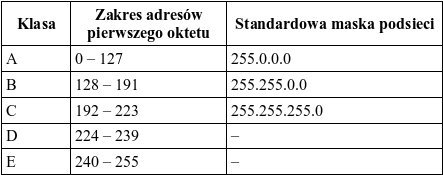
\includegraphics[scale=0.65]{ip-classes.jpg}
					\caption{Klasy IP}
				\end{figure}
			\subparagraph{Adresy klasy A} przeznaczone są dla dużych sieci. Pierwszy bit oktetu w którym zawarty jest adres sieci jest równy 0. W związku z tym adresy sieci mogą przyjmować wartości od 0 do 127. Sieci 0 i 127 są zarezerwowane, więc do wykorzystania pozostają sieci od 1 do 126. W każdej sieci należącej do klasy A możemy wyodrębnić 16777216 adresów (liczba urządzeń będzie o 2 mniejsza, ale o tym w dalszej części artykułu). Klasa 127.0.0.0 wykorzystywana jest na potrzeby pętli zwrotnej, tj. umożliwia wysyłanie pakietów do samego siebie. Maska standardowa dla tej klasy to 255.0.0.0.
			
			\subparagraph{Adresy klasy B} przeznaczone są do sieci średniej wielkości. Adres sieci zawarty jest w dwóch oktetach. Pierwsze dwa bity pierwszego oktetu wynoszą 10. W każdej sieci należącej do tego klasy można wyróżnić 65536 adresów (65534 urządzenia). Do tej klasy należą adresy sieci od 128 do 191 w ujęciu dziesiętnym. Maska standardowa dla tej klasy to 255.255.0.0.
			
			\subparagraph{Adresy klasy C} przeznaczone są dla małych sieci, gdyż każda sieć może posiadać „jedynie” 256 adresów (254 urządzenia). Na adres sieci w sieciach należących do tej klasy przeznaczone są 3 oktety. Pierwsze trzy bity adresu wynoszą 110, w związku z tym do klasy tej należą adresy od 192 do 223 dziesiętne. Maska standardowa dla tej klasy to 255.255.255.0.
			
			\subparagraph{Klasa D} została zarezerwowana na potrzeby rozsyłania grupowego przy użyciu adresów IP. Adres należący do tej klasy umożliwia przekierowanie pakietów do zdefiniowanej wcześniej grupy odbiorców. Dzięki temu możliwe jest przesłanie danych równocześnie do wielu odbiorców. Adresy tej klasy wykorzystywane są np. przez protokoły routingu. Pierwsze cztery bity adresu IP są równe 1110. Adresy należące do tej klasy zawierają się w przedziale od 224 do 239.
			
			\subparagraph{Adresy należące do klasy E} zostały zarezerwowane przez Internet Engineering Task Force na potrzeby badawcze, wobec tego nie są dostępne publicznie. Pierwsze cztery bity adresu klasy E mają wartość 1111, w związku z tym adresy tej klasy zawierają się w przedziale od 240 do 255 dziesiętnie.
			\subsubsection{Prywatne adresy IP}
				Adresy prywatne wg klas:
				\begin{itemize}
					\item Klasa A – 10.0.0.0 – 10.255.255.255 z maską 255.0.0.0
					\item Klasa B – 172.16.0.0 – 172.31.255.255 z maską 255.255.0.0
					\item Klasa C – 192.168.0.0 – 192.168.255.255 z maską 255.255.255.0
				\end{itemize}
			\subsubsection{Rodzaje trasowania protokołu IP}
			\begin{enumerate}
				\item Anycast - dane są wysyłane do (topologicznie) najbliższego odbiorcy
				\item Broadcast - dane wysyła do wszystkich możliwych hostów
				\item Multicast - dane są wysyłane do wielu wybranych hostów (np. do hostów należących
				do jednej grupy)
				\item Unicast - dane są wysyłane do jednego odbiorcy
				\item Geocast - dane są wysyłane do wielu wybranych hostów należących do jednej strefy
				geograficznej
			\end{enumerate}
			
			\newpage\section{Atrybuty bezpieczeństwa informacji.}
				Triada bezpieczeczeństwa CIA - Confidentiality, Integrity, Availability
				\begin{enumerate}
					\item Poufność - osoby nieupoważnione nie mają dostępu do informacji podczas
					przechowywania, przetwarzania i przesyłania (np. zaszyfrowanej wiadomości)
					\item Integralność - zapewnia że wiadomość nie została zmodyfikowana (w trakcie
					przechowywania, transportowania lub przetwarzania)
					\item Dostępność - określa nieprzerwany dostęp do zasobów (w odpowiednio szybkim
					czasie) przez osoby aktualnie mające dostęp (np. osoby ze starej sesji nie mają już
					dostępu) i zapobieganie atakom DoS.
					\item Niezaprzeczalność (nie wlicza się do triady) - podmiot nie może zaprzeczyć że
					wykonał jakąś czynność (np. że użytkownik wysłał wiadomość lub chciał uzyskać
					dostęp do strony poprzez logowanie).
					\item Autentyczność - zapewnia że dane które zostały przyjęte pochodzą od osoby która
					faktycznie jest wysłała (jest zapewnione że nikt się nie podszył wysyłając te dane)
					\item Rozliczalność - polega na rejestrowaniu działań/czynności wykonywanych w
					konkretnym czasie przez dane osoby/procesy (np. Janek logował się na strony +18
					30 maja 2018 o 16:54:43)
				\end{enumerate}
				
			\newpage\section{Składnia podstawowych zapytań języka SQL.}
				\subsubsection{DDL - Data Definition Language}
				\noindent Jak zapamiętać skrót: \\ Definition = DEFINIOWANIE - TWORZENIE STRUKTUR \\
				\noindent W skład DDL wchodzą \verb*|DROP|, \verb*|CREATE| oraz \verb*|ALTER|.
				\begin{itemize}
					\itemsep 0em
					\item \verb*|DROP| - usunięcie struktury
					\begin{verbatim}
						DROP TABLE tabela;
					\end{verbatim}
					\item \verb*|CREATE| - stworzenie struktury
					\begin{verbatim}
						CREATE TABLE tabela(
							kolumna1 typ (rozmiar),
							kolumna2 typ (rozmiar),
							...
						);
					\end{verbatim}
					\item \verb*|ALTER| - modyfikacja struktury. Obejmuje operacje takie jak np. dodanie kolumny do tabeli, zmiana typu danych w kolumnie, usunięcie kolumny.
					\begin{verbatim}
						ALTER TABLE table
						ADD kolumna typ(dlugosc);
					\end{verbatim}
					\begin{verbatim}
						
					\end{verbatim}
				\end{itemize}
				
				
				\subsubsection{DML - Data Manipulation Language}
				\noindent Jak zapamiętać skrót: \\ Manipulation = MANIPULACJA - EDYCJA LUB TWORZENIE REKORDÓW \\
				\noindent W skład DML wchodzą \verb*|INSERT|, \verb*|UPDATE| oraz \verb*|DELETE|.
				\begin{itemize}
					\itemsep 0em
					\item \verb*|INSERT| - dodawanie wierszy
					\begin{verbatim}
						INSERT INTO tabela (kolumna1, kolumna2, ..., kolumna_n)
						VALUES (wartosc1, wartosc2, ..., wartosc_n)
					\end{verbatim}
					Nie trzeba podawać kolumn po nazwie tabeli gdy podamy po pierwsze wszystkie wartości, a po drugie w dobrej kolejności
					
					\item \verb*|UPDATE| - aktualizowanie danych, zmiana
					\begin{verbatim}
						UPDATE tabela
						SET kolumna1 = wartosc, kolumna2 = wartosc2, ...
						WHERE warunek
					\end{verbatim}
					WHERE nie jest konieczny, możemy  go użyć jak chcemy doprecyzować które rekordy mają się zaktualizować
					
					\item \verb*|DELETE| - usuwanie wierszy
					\begin{verbatim}
						DELETE FROM tabela
						WHERE warunek
					\end{verbatim}
					WHERE nie jest konieczny, możemy  go użyć jak chcemy doprecyzować które rekordy mają się skasować
				\end{itemize}
				\subsubsection{DCL - Data Control Language}
				\noindent Jak zapamiętać skrót: \\ Control = KONTROLA = UPRAWNIENIA \\
				\noindent W skład DCL wchodzą \verb*|GRANT|, \verb*|REVOKE| oraz \verb*|DENY|.
				
				\begin{itemize}
					\item \verb*|GRANT| - nadawanie uprawnień do pojedynczych obiektów lub globalnie konkretnemu userowi
					\item \verb*|REVOKE| - odbieranie uprawnień konkretnemu userowi
					\item \verb*|DENY| - zabranianie wykonywania operacji
					\item Składnia jest taka sama dla w/w poleceń:
					\begin{verbatim}
						[GRANT/REVOKE/DENY] operacja1, operacja2, ...
						ON tabela
						TO user
					\end{verbatim}
					Przykład:
					\begin{verbatim}
					GRANT SELECT, INSERT
					ON Fragment
					TO glazik
					\end{verbatim}
				\end{itemize}
				
				\subsubsection{DQL - Data Query Language}
				\noindent Jak zapamiętać skrót: \\ Query = ZAPYTANIA = SELECTY \\
				\noindent W skład DQL wchodzi jedno polecenie: \verb*|SELECT|. Pozwala wybierać wiersze z bazy danych. Składnia:
				\begin{verbatim}
					SELECT kolumny 
					FROM tabele 
					WHERE warunek
					GROUP BY kolumna
					HAVING warunek
					ORDER BY ... DESC/ASC;
				\end{verbatim}
				Dodatkowe klauzule \verb*|SELECT|:
				\begin{itemize}
					\itemsep 0em
					\item \verb*|ORDER BY| - sortowanie wyników względem np. kolumny
					\item \verb*|ASC| oraz \verb*|DESC| - dodawane po sortowaniu, wybieramy czy ma być ascending czy descending
					\item \verb*|GROUP BY| - grupowanie wyników względem danej kolumny
					\item \verb*|HAVING| - filtrowanie grup, działa podobnie do WHERE. WHERE oraz HAVING mogą występować jednocześnie w zapytaniu.
				\end{itemize}
				
			\newpage\section{Metodyki zwinne (agile).}
				\subparagraph{Programowanie zwinne (agile)} - są to metodyki wytwarzania oprogramowania które są
				oparte na programowaniu iteracyjno-przyrostowym oraz na obserwowaniu czy wymagania
				nie ewolują.
				
				Cechy:
				\begin{itemize}
					\item przeznaczony głównie dla małych zespołów programistycznych
					\item w zespołach nie występuje hierarchia
					\item zespoły same się organizują
					\item komunikacja jest jednym z głównych elementów podczas produkcji oprogramowania
					\item szybkie wytwarzanie oprogramowania (i dobrej jakości)
					\item oprogramowanie jest dostarczane cyklicznie
					\item mała ilość dokumentacji
				\end{itemize}
			
				Manifest Agile (ważniejsze > mniej ważne [ale występuje]):
				\begin{itemize}
					\item Ludzie i interakcje > Procesy i narzędzia
					\item Działające oprogramowanie > Obszerna dokumentacja
					\item Współpraca z klientem > Formalne ustalenia
					\item Reagowanie na zmiany > Podążanie za planem
				\end{itemize}
		
				Etapy Agile:
				\begin{enumerate}
					\item Planowanie - zbieranie wymagań klienta i ich analiza (kluczowa jest umiejętność
					dobrej komunikacji z klientem)
					\item Projektowanie - polega na przemyśleniu jak wykonać zaplanowany element
					\item Programowanie
					\item Testowanie
					\item Informacja zwrotna - zgłaszanie niewykrytych błędów, nowych pomysłów i zmian
					wymagań klienta
				\end{enumerate}
			
				\subsubsection{Metodyki zwinne}
				\begin{enumerate}
					\item XP (eXtreme Programming)
					\begin{itemize}
						\item stosowany w małych i średnich projektach “wysokiego ryzyka” (czyli takich
						gdzie nie wiadomo do końca jak zrealizować dany cel)
						\item tutaj najpierw są pisane testy, a potem program
						\item na początku projekt ma za zadanie spełniać minimalne wymagania lecz
						potem jest rozwijany i z każdą iteracją (co kilka tygodni) następuje kontakt z
						klientem który wyraża swoja opinię (informację zwrotną)
						\item występuje kontakt klient-programista
						\item podstawą jest dobra komunikacja ustna w zespole (brak dokumentacji)
						\item programiści pracują parami (jeden pisze, a drugi poprawia i komentuje; po
						jakimś czasie następuje zamiana)
						\item kod jest wspólny dla wszystkich i każdy może coś zmienić
						\item brak dokładnej specyfikacji wymagań
						\item iteracja posiada 4 etapy (wykonywane równolegle, a nie po sobie) :
						Planowanie, Projektowanie, Programowanie, Testowanie					
					\end{itemize}
					\begin{figure}[h!]
						\centering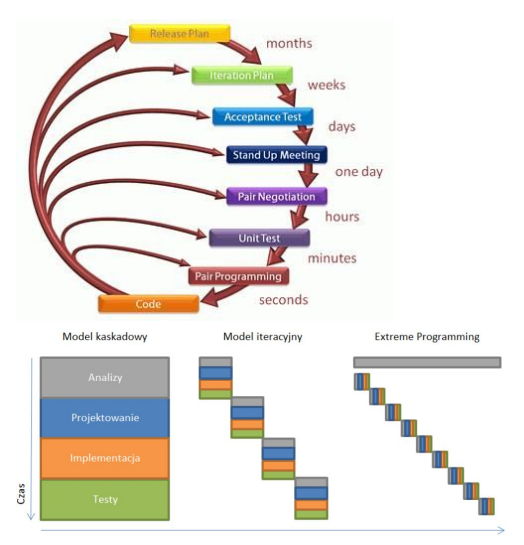
\includegraphics[scale=0.8]{xp.png}
					\end{figure}
				
					\item Scrum
					\begin{itemize}
						\item iteracje wytwarzania oprogramowania są nazywane Sprintami (iteracja trwa
						najwyżej miesiąc)
						\item każdy sprint dodaje nową funkcjonalność (jak w większości metodyk)
						\item zespół się sam organizuje (podobnie jak w XP)
						\item występują tutaj codzienne 15 minutowe spotkania całego zespołu w celu
						omówienia projektu (co kto zrobił, co zamierza zrobić)
						\item Podczas produkcji występują 3 role:
						\begin{itemize}
							\item Development Team - to grupa od 3 do 9 osób która tworzy produkt
							\item Product Owner - osoba reprezentująca klienta (bierze ciągły udział
							podczas produkcji
							\item Scrum Master - osoba która wspiera zespół, pomaga gdy zespół o to
							poprosi, interweniuje gdy trzeba, pracuje z Product Ownerem (to taki
							opiekun)
						\end{itemize}
						\item proces wytwórczy:
						\begin{itemize}
							\item zbieranie listy wymagań i określanie cech systemu (czyli
							funkcjonalności istotnych z punktu widzenia klienta)
							\item Product Owner przedstawia priorytety i główny cel (z tych wymagań)
							\item (początek sprintu) wybieranie zadań o najwyższym priorytecie
							\item tworzenie oprogramowania (programiści sami wybierają które
							zagadnienia chcą robić [no z tych priorytetowych oczywiście]) z
							udziałem Product Ownera i występujące codzienne 15 minutowe
							spotkania
							\item (koniec sprintu) prezentowanie wyników ze sprintu
						\end{itemize}
					\end{itemize}
				\begin{figure}[h!]
					\centering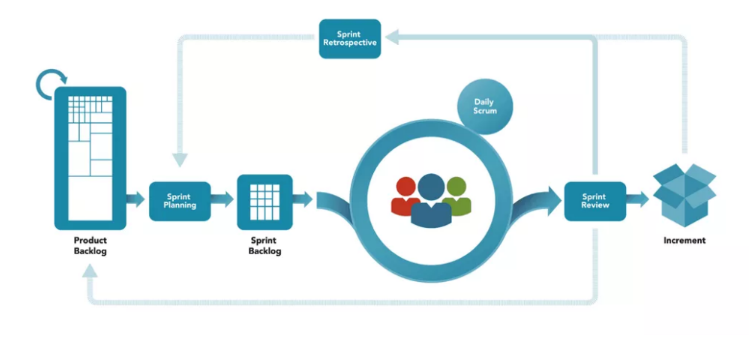
\includegraphics[scale=0.7]{scrum.png}
				\end{figure}
				\item TDD (Test-driven development)
				\begin{itemize}
					\item polega on na tym że na początku są pisane testy, a potem kod
					\item przydatny dla większych projektów (dla maych to jest strata czasu z pisaniem
					tych testów)
					\item etapy cyklu tworzenia oprogramowania:
					\begin{itemize}
						\item napisanie testów (które nie przechodzą przy braku implementacji)
						\item napisanie kodu które przejdzie test
						\item refaktoryzacja kodu
					\end{itemize}
					\item pisanie testów na początku zmniejsza ryzyko występowania błędów
					\item to jest technika “pierwsze testy, a potem kod” zmniejszający ryzyko
					występowania błędu, a gdy jest odwrotnie to nie dość że trzeba szukać błędu
					to i ilość kodu jest większa (od powstania błędu)
				\end{itemize}
				\begin{figure}[h!]
					\centering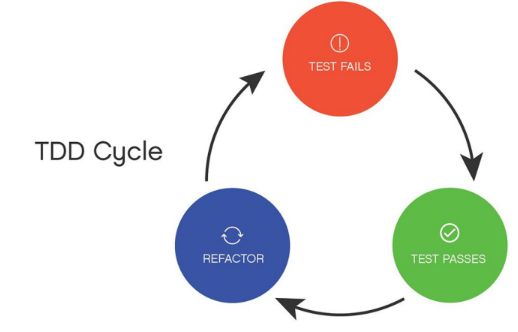
\includegraphics[scale=0.6]{tdd.png}
				\end{figure}
				\end{enumerate}
\end{document}